\section{Viewing and Cleaning the Data}
\label{sec:clean}
\fix{George's section: The two views of GPU life: by SN and by
  location, its use in cleaning data, etc.}

A typical GPU data record produced by the methods in the last section
is of the form shown in Fig.~\ref{fig:dataraw},
\begin{figure}
{\small
\begin{verbatim}
0323812007945 | c17-4c1s3n1 | 01/10/2013 02:54:45 | 02/02/2013 11:32:29
 | c13-1c1s3n3 | 01/21/2014 21:10:42 | 08/01/2017 02:15:02
 | c0-1c1s3n3 | 10/11/2013 15:57:33 | 10/12/2013 22:09:31
 | c21-1c2s5n0 | 03/19/2013 15:48:11 | 05/29/2013 11:54:11
0325216047736 | c18-4c1s5n1 | 03/07/2017 02:15:01 | 03/12/2019 03:19:11
0323812008856 | c5-4c0s7n0 | 01/10/2013 02:54:45 | 01/25/2013 15:29:58
 | c0-6c1s7n2 | 10/21/2013 14:28:19 | 10/28/2013 17:52:44
 | c3-3c1s5n0 | 05/29/2013 11:54:11 | 05/29/2013 11:54:11
 | c23-6c1s7n2 | 01/21/2014 21:10:42 | 11/02/2018 14:42:34
 | | DBE | 11/02/2018 14:42:34
\end{verbatim}
}
\caption{Raw data.}
\label{fig:dataraw}
\end{figure}
\noindent where records for three GPUs are shown. Each record starts
with a serial number and locations are coded with {\tt c{\it
    col-row}c{\it cage}s{\it slot}n{\it node}}. The first GPU record
shows installation in locations {\tt c17-4c1s3n1}, {\tt c21-1c2s5n0},
{\tt c0-1c1s3n3}, with periods off the system, and finally in {\tt
  c13-1c1s3n3}, where it stays until August 1, 2017, after which it is
not seen again. The second is intalled in location {\tt c18-4c1s5n1},
where it stays until the last data collection date on March 3, 2019,
at 3:19:11 AM. The third GPU is first installed in locations {\tt
  c5-4c0s7n0}, {\tt c3-3c1s5n0},{\tt c0-6c1s7n2}, {\tt c23-6c1s7n2},
where a ``DBE'' is observed on November 2, 2018, and it is not seen
again.

As we need to recover durations from this data, correct processing
involves time adjustments for switching between daylight saving time
and standard time. We perform this by setting a reference time zone
(Eastern time) and converting all date-times from strings into
date-time variables \fix{(is there a name for this?)} with the R
\pkg{lubridate} package \cite{lubridate}, which enables appropriate
date arithmetic.

\fix{Other processing:} enable missing values, and create some new
variables. The event is “life” when both insert and remove are
present, “life0” when insert = remove, otherwise it is whatever string
is in insert, which is “DBE” or “Off The BUS”. Also separate location
into its components and fill in (repeat) serial numbers and locations
for all records.

Reduce to only “life” records and mark them with ending DBE, OTB,
“out”, or none events. The result is just insert and remove with event
marks to indicate DBE or OTB or “out” (last seen). bad indicates that
a DBE or OTB occurred yet the GPU was not taken out. For a first cut,
keep the bad ones in. Also keep duration to later aggregate into full
life times.

Next, aggregate into one record per serial number with total life time
and first insert time. For proper censoring treatment: Indicate if
event occurred or still in service: out = fail, dbe = fail, otb =
fail, NA = right censored (still in service). Add some other
variables, such as GPU in single location or moved one or more times,
mark new\_batch group, etc. to use in modeling later.

A plot of the life of 100 random GPUs on Titan after cleaning the data:
\begin{description}
\item[starts:] black dots (gray for zero lifetime)
\item[lifetimes:] black lines
\item[DBEs:] red triangles
\item[Off The BUS:] blue triangles
\item[Last seen:] black ]
\item[overlaps:] red square on left when they exist
\end{description}

\begin{figure}[ht]
  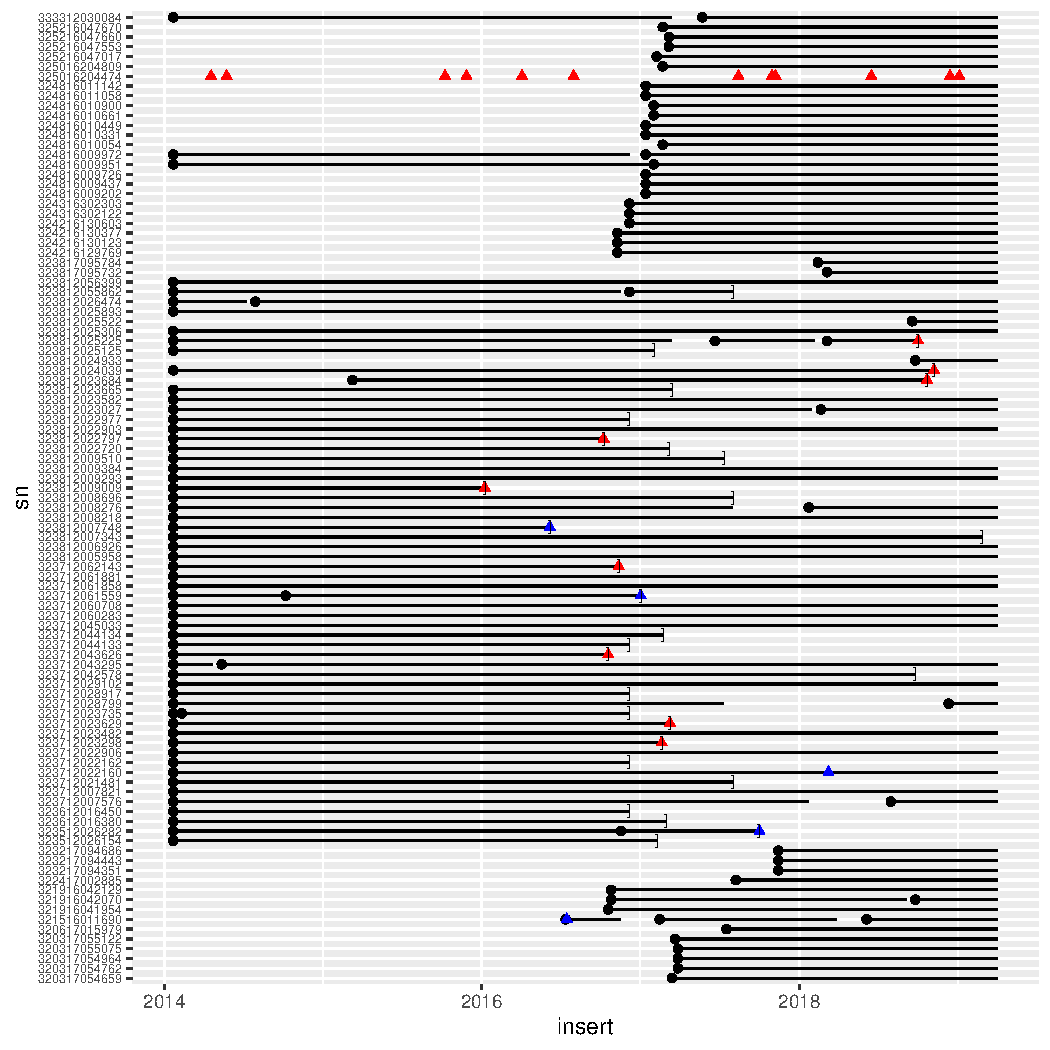
\includegraphics[width=6in]{sn.pdf}
  \caption{GPU serial number view of life and failures.}
\end{figure}



\begin{figure}[ht]
  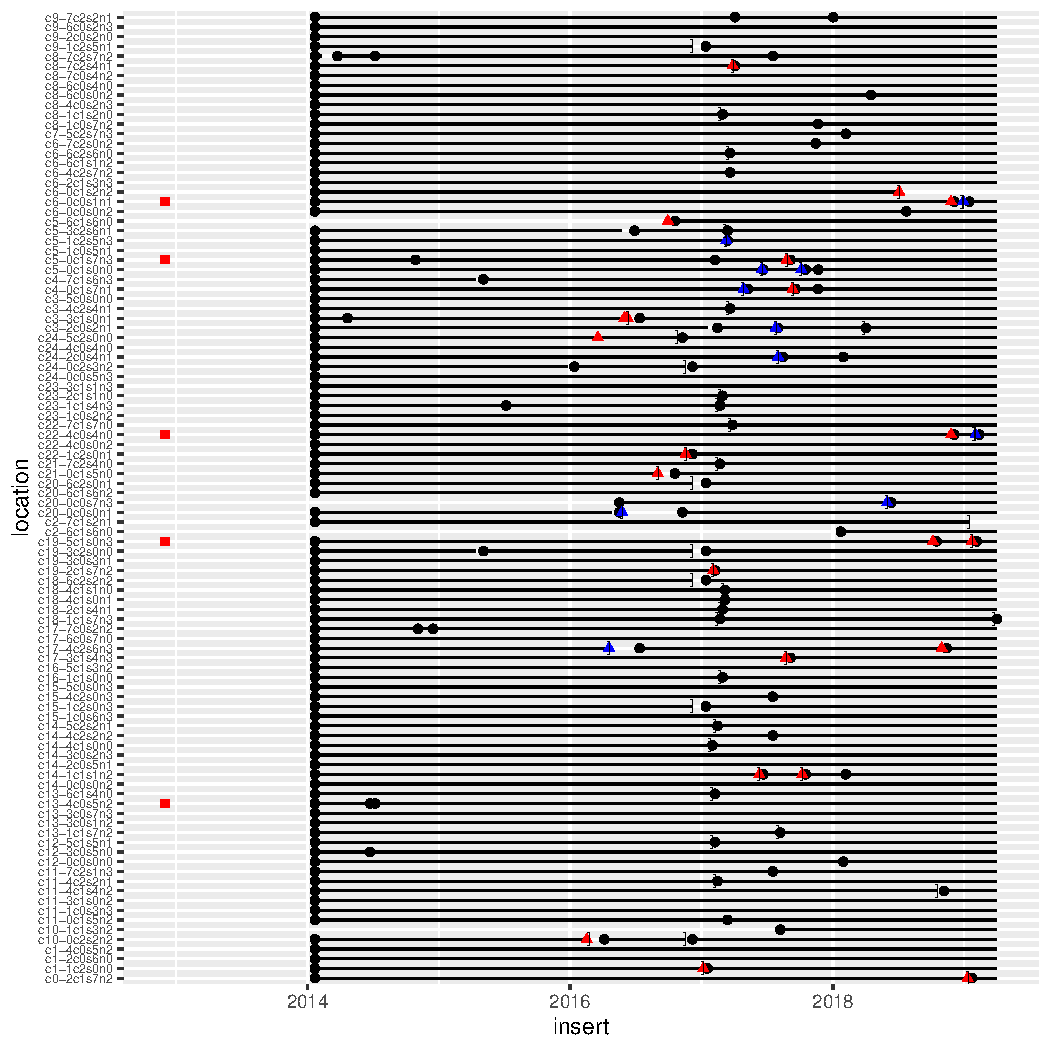
\includegraphics[width=6in]{location.pdf}
  \caption{GPU location view of life and failures.}
\end{figure}

